\section{Ruby on Rails} % (fold)
\label{tech:sec:ruby_on_rails}
David Hansson and \textit{37signals} began working on a web-based project management tool oriented towards small teams in 2003. They initially started by using PHP but soon became frustrated by many of the language's shortcomings. Hansson soon gave up on this language and started implementing what today is known as \textit{Basecamp} in pure Ruby. While developing the application, he noticed that a lot of its code could be extracted into a framework for future use with other applications. Hansson decided to release his framework to the public in July 2004 and Ruby on Rails was born~\cite{railssolutions}.

Rails started to become more popular and mature over time and applications like Twitter, YellowPages, Hulu, Scribd and GitHub currently use this framework.

Ruby on Rails has three main principles which motivated its creation~\cite{agile_webdevelopment_with_rails, ruby_on_rails_principles}:
\begin{description}
\item[Convention over configuration.] In Rails, everything has a default configuration. The only exception is the database connection data. This way, developers only need to specify when they want to use unconventional configurations. This way, Rails offers simplicity while retaining its flexibility.
\item[Don't Repeat Yourself.] Also known as DRY, this practice implies that the similar pieces of code do not exist in separate locations. Every piece of knowledge is unique, definite and has a relevant representation. This simplifies modifications by the avoidance of having to change the same logic in different parts of the project, allowing the applications to keep a high level of consistency. 
\item[Model-View-Controller.] Rails follows the MVC architecture pattern, keeping the source code well organized by clearly separating the code according to its purpose. The \textit{Model} is responsible for maintain the state of the application, specifying the constraints its related data has to obey to. The \textit{Controller} receives the users' input, interacts with the model and finally renders a view page as the result. The \textit{View} can have multiple formats, from JSON to XML, and is essentially what is displayed to the users. This principle's schema is presented in figure~\ref{fig:mvc}.
\begin{figure}[h]
  \centering
    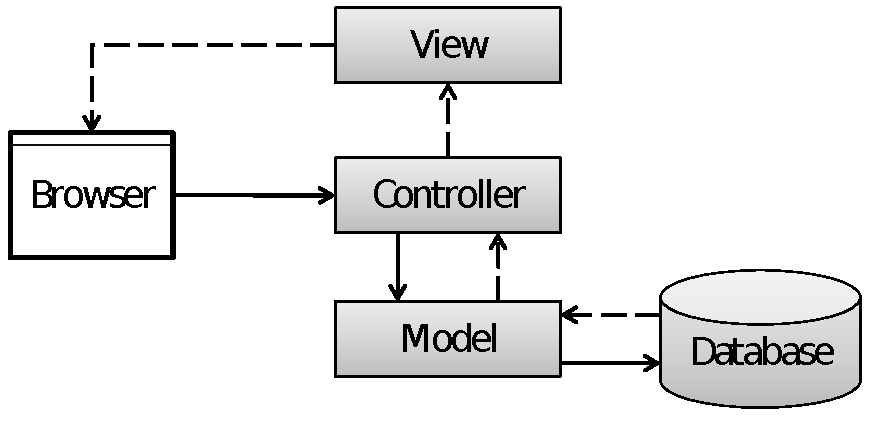
\includegraphics[width=0.75\textwidth]{mvc}
  \caption{Model-View-Controller architectural pattern}
  \label{fig:mvc}
\end{figure}\\
\end{description}
Rails' functionality can be altered and extended with plugins. While being a full stack web framework, Rails does not aim to include every single feature. However, it has been built with a highly extensible infrastructure and it has a considerable set of plugins nowadays~\cite{rails_magazine_1}.


\subsection{Rails 2}
Rails 2 was first released in 2007 and is currently in version 2.3, released at the beginning of 2009. Throughout these 2 years the framework was improved by many contributors, aside from the usual suspects --- Rails' core team at \textit{37signals}. The framework is essentially divided in six essential classes~\cite{ruby_on_rails_principles, rails23_release_notes}:
\begin{description}
\item[ActionMailer] allows the application to send emails using a mailer model and views.
\item[ActionPack] splits the response in two:  a request for the controller to handle the login and a template rendering part for the view to handle.
\item[ActiveRecord] is responsible for object handling and their database representation. Objects are directly linked to the database, so modifying them will modify the table definition they are associated with.
\item[ActiveResource] corresponds to objects that represent the application's RESTful resources as manipulatable Ruby objects.
\item[ActiveSupport] is a collection of various utility classes and standard library extensions.
\item[ActionMailer] is a framework for designing email-service layers.
\end{description}
There are a lot more classes that inherit from those listed above.


\subsection{Rails 3}
\label{tech:sec:ruby_on_rails:rails3}
Rails 3 is currently in development and a beta release is scheduled for the 5$^{th}$ of February of 2010. Most of Rails' code has been refactored and this release's main goals were concerned with improved component decoupling and performance~\cite{rails3_great_decoupling}. 

As of component decoupling, a great deal of work has been done and impressive goals have been achieved~\cite{vaporware_to_awesome}. Most of Rails' components are agnostic now, having standard interfaces for communication with each other. The key concept is that a component is agnostic to whom is interacting with it. For this to happen interaction procedures have been developed, providing each of Rails' components with a standard interface.

The decoupling process also allowed for improved modularity, permitting Rails' component separation. ActionController, for instance, has been split into ActionDispatch, ActionController and AbstractController~\cite{vaporware_to_awesome}. There was a lot of work on explicitly handling each component's internal dependencies. This enables the developer to carefully select which modules he needs in his Rails application without caring about including the modules it depends on as well. In previous versions of Rails, one had to import the top-level modules. The alternative was to parse the source code of the framework to find its internal dependencies in order to import all necessary modules. Applications are now able to only load the modules they really need thus becoming faster and lighter.
While this improved modularity also had its impact on performance, some effort was also put into common Rails bottlenecks like partial and collection rendering~\cite{vaporware_to_awesome}, among some other optimized sections.

